\begin{Schunk}
\begin{Sinput}
> library("Ham94", lib.loc = "../../../library")
\end{Sinput}
\end{Schunk}
Page 376 describes an application of Kalman filtering to business cycles by James Stock and Mark Watson.

This can be implemented in two steps.  The first is to implement the Kalman algorithm as described in the text.  The
following function follows the notation in Chapter 13.
\begin{Schunk}
\begin{Sinput}
> kalman <- function(H, R, F, x, A, y, Q, xi.1.0, P.1.0) {
+     T <- dim(x)[[2]]
+     P.t.t_1 <- array(dim = c(dim(P.1.0), T + 1))
+     P.t.t_1[, , 1] <- P.1.0
+     P.t.t <- array(dim = c(dim(P.1.0), T))
+     K.t <- array(dim = c(dim(H), T))
+     xi.t.t_1 <- array(dim = c(length(xi.1.0), T + 1))
+     xi.t.t_1[, 1] <- xi.1.0
+     xi.t.t <- array(dim = c(length(xi.1.0), T))
+     L <- 0
+     for (tt in 1:T) {
+         V <- solve(t(H) %*% P.t.t_1[, , tt] %*% H + R)
+         K.t[, , tt] <- P.t.t_1[, , tt] %*% H %*% V
+         P.t.t[, , tt] <- P.t.t_1[, , tt] - K.t[, , tt] %*% t(H) %*% 
+             P.t.t_1[, , tt]
+         P.t.t_1[, , tt + 1] <- F %*% P.t.t[, , tt] %*% t(F) + 
+             Q
+         w <- y[, tt] - t(A) %*% x[, tt] - t(H) %*% xi.t.t_1[, 
+             tt]
+         xi.t.t[, tt] <- xi.t.t_1[, tt] + K.t[, , tt] %*% w
+         xi.t.t_1[, tt + 1] <- F %*% xi.t.t[, tt]
+         L <- L - 1/2 * dim(y)[[1]] * log(2 * pi) + 1/2 * log(det(V)) - 
+             1/2 * t(w) %*% V %*% w
+     }
+     xi.t.T <- array(dim = c(length(xi.1.0), T))
+     xi.t.T[, T] <- xi.t.t[, T]
+     P.t.T <- array(dim = c(dim(P.1.0), T))
+     P.t.T[, , T] <- P.t.t[, , T]
+     for (tt in (T - 1):1) {
+         Jt <- P.t.t[, , tt] %*% t(F) %*% solve(P.t.t_1[, , tt + 
+             1])
+         xi.t.T[, tt] <- xi.t.t[, tt] + Jt %*% (xi.t.T[, tt + 
+             1] - xi.t.t_1[, tt + 1])
+         P.t.T[, , tt] <- P.t.t[, , tt] + Jt %*% (P.t.T[, , tt + 
+             1] - P.t.t_1[, , tt + 1]) %*% t(Jt)
+     }
+     list(xi.t.t = xi.t.t, xi.t.t_1 = xi.t.t_1, P.t.t = P.t.t, 
+         P.t.t_1 = P.t.t_1, K.t = K.t, log.likelihood = L, xi.t.T = xi.t.T, 
+         P.t.T = P.t.T)
+ }
\end{Sinput}
\end{Schunk}
The second is to specify the state space model as described on pp376-377 and estimate the parameters
via maximum likelihood.  Data for this analysis is consumption and income data form dataset "coninc" in log differences.
\begin{Schunk}
\begin{Sinput}
> data(coninc, package = "Ham94")
> YGR <- diff(log(coninc$GYD82))
> CGR <- diff(log(coninc$GC82))
> y <- t(cbind(YGR - mean(YGR), CGR - mean(CGR)))
\end{Sinput}
\end{Schunk}
The following helper function converts the parameters from a vector of labeled
components into the correct inputs for the filter as shown in equations [13.1.28], [13.1.29], and [13.1.30].
\begin{Schunk}
\begin{Sinput}
> THETA <- c(phic = 0.9, phi1 = 0.9, phi2 = 0.9, g1 = 0.5, g2 = 0.5, 
+     sigc = 0.05^0.5, sig11 = 0.05^0.5, sig22 = 0.05^0.5, r11 = sd(YGR), 
+     r22 = sd(CGR))
> theta.y.to.params <- function(THETA, y) {
+     params <- list(F = diag(THETA[c("phic", "phi1", "phi2")]), 
+         Q = diag(THETA[c("sigc", "sig11", "sig22")]^2), H = rbind(THETA[c("g1", 
+             "g2")], diag(2)), R = diag(THETA[c("r11", "r22")]^2), 
+         A = diag(c(0, 0)), x = c(1, 1) %o% rep(1, dim(y)[[2]]), 
+         xi.1.0 = c(0, 0, 0))
+     c(params, list(P.1.0 = array(solve(diag(length(params$xi.1.0)^2) - 
+         params$F %x% params$F, as.vector(params$Q)), c(length(params$xi.1.0), 
+         length(params$xi.1.0)))))
+ }
\end{Sinput}
\end{Schunk}
The objective function is the log.likelihood obtained from the Kalman iteration.
\begin{Schunk}
\begin{Sinput}
> objective <- function(THETA, y) {
+     params <- theta.y.to.params(THETA, y)
+     kalman(params$H, params$R, params$F, params$x, params$A, 
+         y, params$Q, params$xi.1.0, params$P.1.0)$log.likelihood
+ }
> optimizer.results <- optim(par = THETA, fn = objective, gr = NULL, 
+     y = y, control = list(trace = 0))
\end{Sinput}
\end{Schunk}
Finally calculate the smoothed results based on the ML estimated parameters.
\begin{Schunk}
\begin{Sinput}
> params <- theta.y.to.params(optimizer.results$par, y)
> smoothed.results <- kalman(params$H, params$R, params$F, params$x, 
+     params$A, y, params$Q, params$xi.1.0, params$P.1.0)
> smoothed.data <- smoothed.results$xi.t.T[1, ]
\end{Sinput}
\end{Schunk}
The results of the smoothed inference are shown below.
\begin{center}
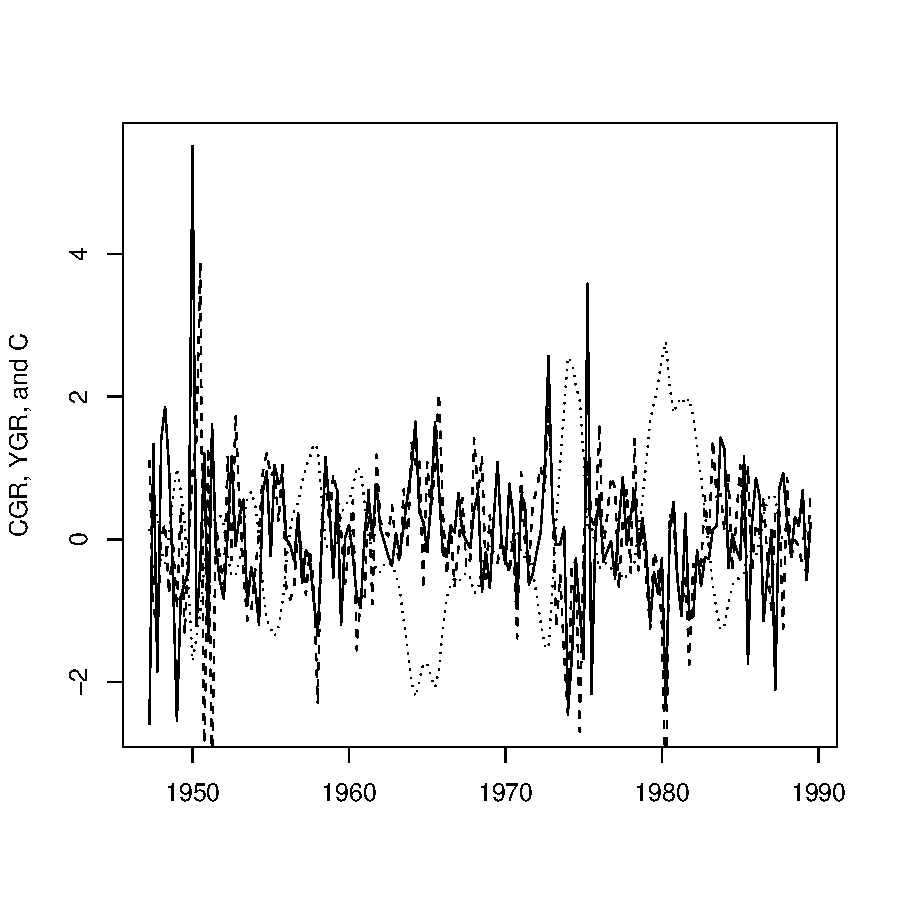
\includegraphics{p376-007}
\end{center}
\subsection{R facilities for Kalman Filtering}
There are several different packages in R for Kalman filtering, some that provide univariate support,
others multivariate support.  For example, package FKF is a fast implementation, but there are others. One key
aspect of using such packages is specifying an interface to allow for time varying inputs, and providing results
under those conditions.  Some packages use caller supplied functions, others check for dimensions of (up to three
dimensional) arrays, etc.

For example, a simple implementation of the example on page 382 using function "kalman" above might look like:
\begin{Schunk}
\begin{Sinput}
> sigmasq <- 2
> params <- list(F = array(c(0, 1, 0, 0), c(2, 2)), Q = diag(c(sigmasq, 
+     0)), H = array(c(1, 0.8), c(2, 1)), R = array(0, c(1, 1)), 
+     A = array(0.5, c(1, 1)), x = 1 %o% rep(1, 5), y = 1 %o% c(1, 
+         seq(0.5, 4)), xi.1.0 = c(0, 0))
> params <- c(params, list(P.1.0 = array(solve(diag(length(params$xi.1.0)^2) - 
+     params$F %x% params$F, as.vector(params$Q)), c(length(params$xi.1.0), 
+     length(params$xi.1.0)))))
> myResults <- kalman(params$H, params$R, params$F, params$x, params$A, 
+     params$y, params$Q, params$xi.1.0, params$P.1.0)
\end{Sinput}
\end{Schunk}
We can perform the some operations using package FKF with a slight alteration of the function arguments.
In particular, many of the arguments using an outer product as a quick way to convert them into a structure
of one additional dimension, with the length of the additional dimension being 1.  This is a convenient calling convention to specifying a *non* time varying parameter.  If the
parameter *were* time varying then the full extra dimension would be used.
For example, the F matrix can
be time varying in FKF (called Tt).  A call exploiting this would then have a vector of two dimensional F matrices, one
for each time index, i.e. a three dimensional array.  If F is not time varying, (as in the case of the simple
example above) then a three dimensional array with the
third dimension being of length 1 is used.
\begin{Schunk}
\begin{Sinput}
> fkfResults <- FKF::fkf(a0 = params$xi.1.0, P0 = params$P.1.0, 
+     dt = rep(0, length(params$xi.1.0)) %o% 1, Tt = params$F %o% 
+         1, HHt = params$Q %o% 1, ct = t(params$A) %*% params$x, 
+     Zt = t(params$H) %o% 1, GGt = params$R %o% 1, yt = params$y, 
+     check.input = TRUE)
\end{Sinput}
\end{Schunk}
The results can be confirmed by examing the output:
\begin{Schunk}
\begin{Sinput}
> print(myResults$xi.t.t)
\end{Sinput}
\begin{Soutput}
          [,1]       [,2]        [,3]     [,4]     [,5]
[1,] 0.3048780 -0.1951600  1.02502699 1.100137 2.031900
[2,] 0.2439024  0.2439500 -0.03128374 1.124828 1.210125
\end{Soutput}
\begin{Sinput}
> print(fkfResults$att)
\end{Sinput}
\begin{Soutput}
          [,1]       [,2]        [,3]     [,4]     [,5]
[1,] 0.3048780 -0.1951600  1.02502699 1.100137 2.031900
[2,] 0.2439024  0.2439500 -0.03128374 1.124828 1.210125
\end{Soutput}
\end{Schunk}

